\section{Przeglądanie ofert}

Zarówno klienci, jak i wykonawcy posiadają możliwość przeglądania ofert, lecz w nieco innym kontekście. Pierwsi mogą zobaczyć te, które zostały złożone do utworzonych przez siebie zleceń, a drudzy te, które sami złożyli.

W celu jasnego wyrażenia stanu ofert postanowiono wprowadzić dla nich  cztery  możliwe statusy: nowe, anulowane, w realizacji, wykonano. Stanowią one sposób na etykietowanie ofert oraz zapewniają spójny sposób ich postrzegania przez obie strony. Zostały one stworzone z myślą o wykorzystaniu w następujący sposób:

\begin{itemize}
    \item nowe - jedynie dla nowo utworzonych ofert;
    \item anulowane - gdy współpraca została porzucona;
    \item w realizacji - gdy współpraca została potwierdzona;
    \item wykonano - gdy usługa została wykonana.
\end{itemize}

% Założono, że każda oferta będzie posiadała status, na będzie jasno wyrażał etap na którym znajdują się prace. Założono istnienie następujących statusów: nowe, anulowane, w realizacji, wykonano. Status nowej oferty jest przyznawany nowo stworzonym, którym nie zdążono przypisać jeszcze innego. Jeżeli klient lub wykonawca postanowi zrezygnować ze współpracy, to może zmienić status na \enquote{anulowane}, a w przeciwnym wypadku na \enquote{w realizacji}. W chwili, gdy usługa zostanie wykonana to status powinien zostać zmieniony przez jednego z nich na \enquote{wykonane}. Takie podejście znacznie ułatwia pracę z duża liczbą ofert i umożliwia filtrowanie po statusie, które zastosowano.

Na rysunku \ref{fig:offers-client} zamieszczono ekran ofert, które zostały zgłoszone do utworzonego przez klienta zlecenia. Są przedstawione w postaci listy, której każdy element zawiera podstawowe informacje o wykonawcy, ostatnią wiadomość z chatu oraz status. Jeśli istnieją nieodczytane wiadomości lub oferta jest nowa, to zostaje ona wyróżniona. Dostępna jest możliwość filtrowania opisywanej listy przy pomocy statusów ofert. Klient, jako twórca zlecenia, ma również możliwość zobaczenia planowanej daty jego zamknięcia oraz wykonania tego wcześniej.

\begin{figure}[ht!]
  \captionsetup[subfigure]{justification=centering}
  \centering
  \begin{subfigure}[t]{0.32\textwidth}
    \centering
    \fbox{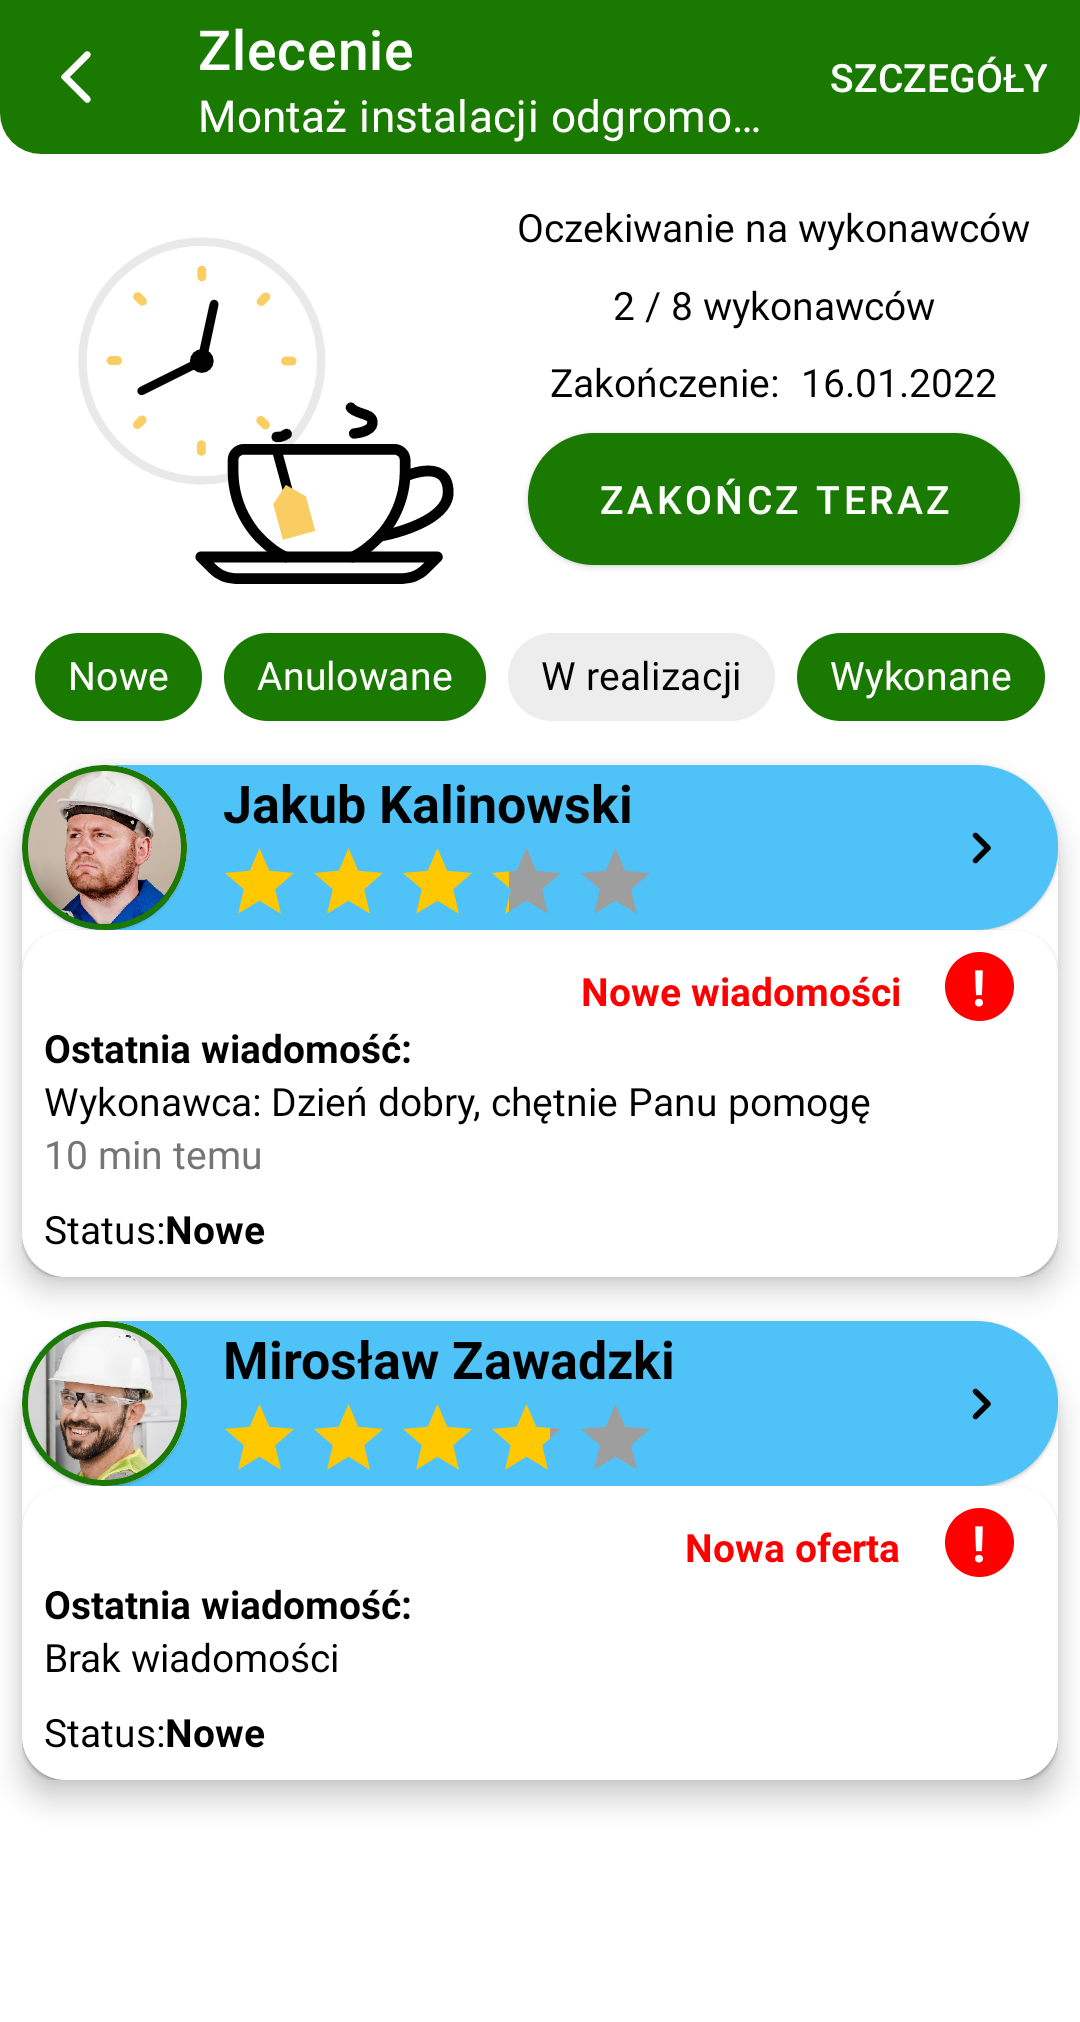
\includegraphics[width=0.97\linewidth]{screens/client_offers_open.png}}
    \caption{Widok otwartego zlecenia}
  \end{subfigure}
  \begin{subfigure}[t]{0.32\textwidth}
    \centering
    \fbox{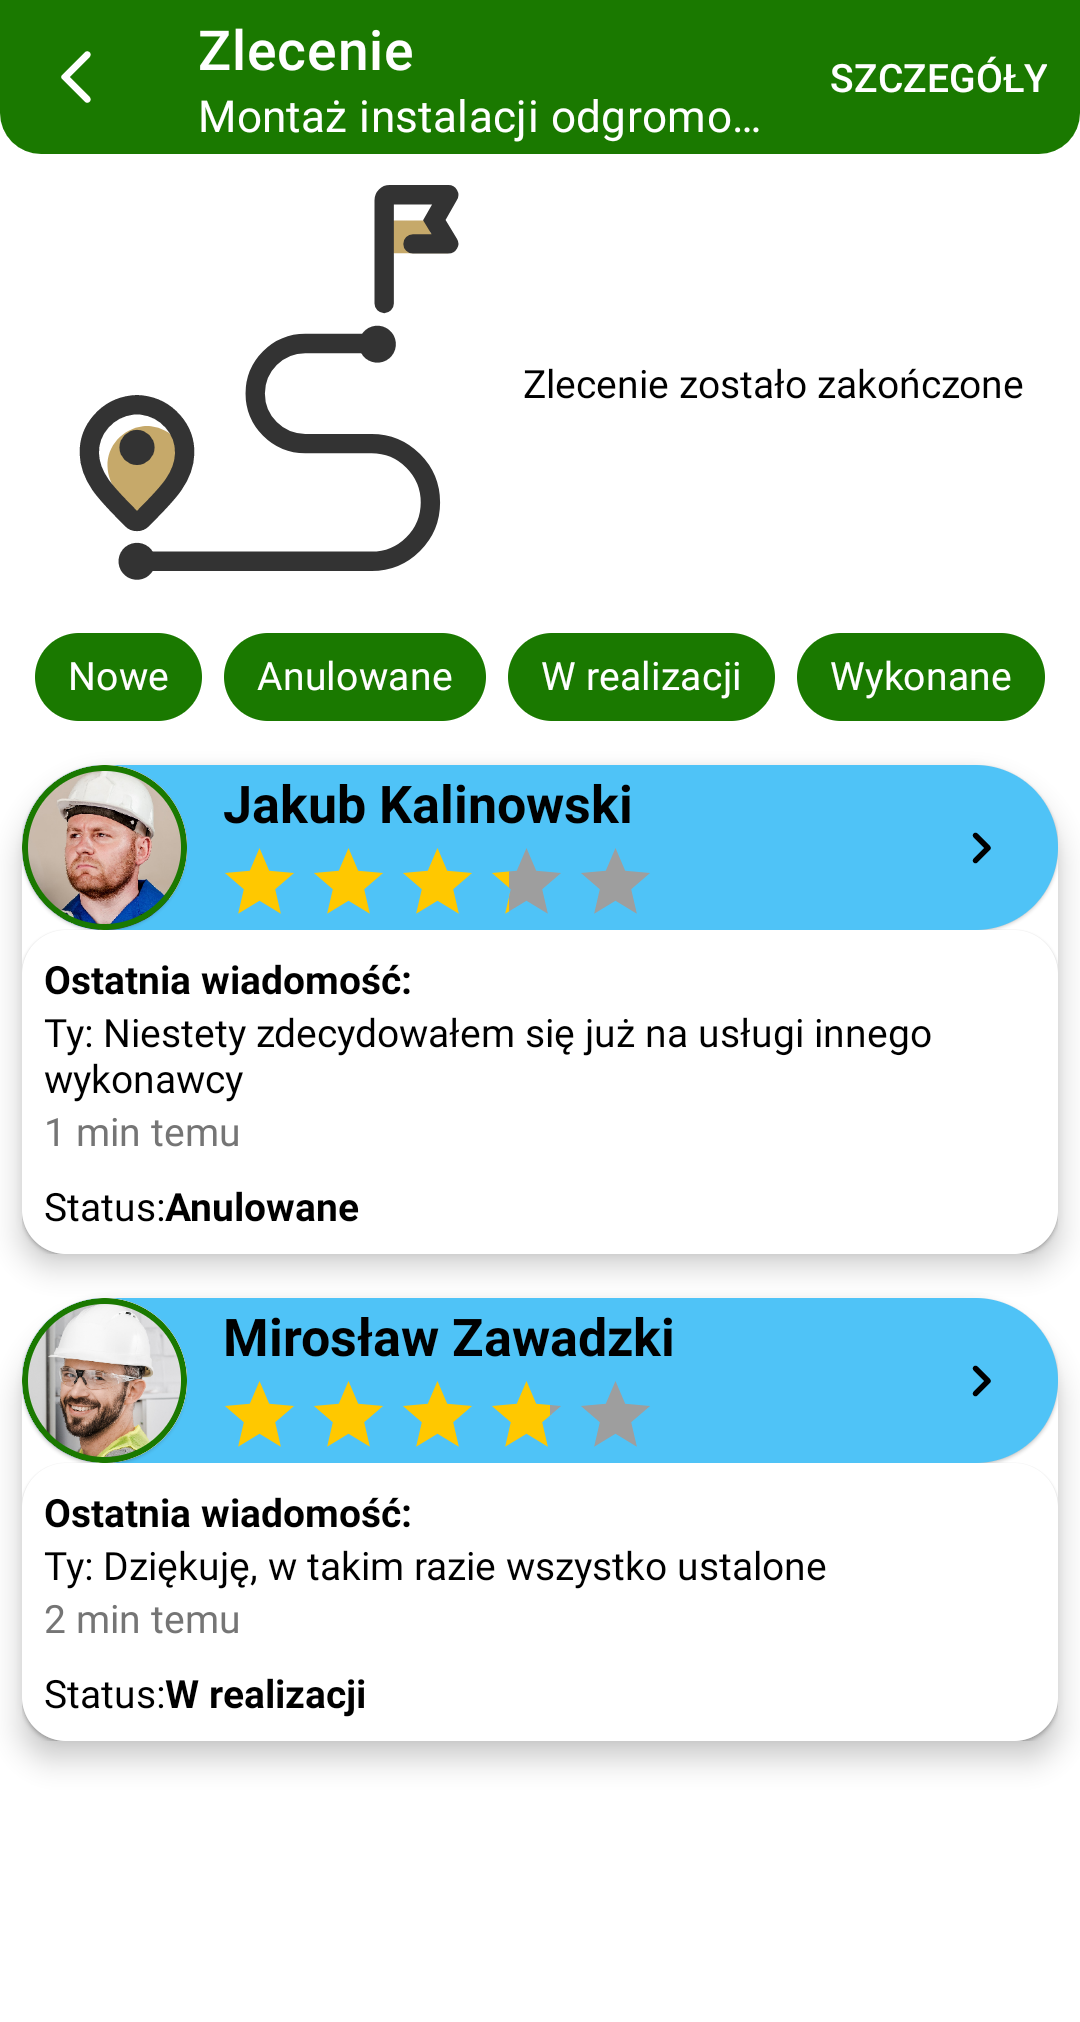
\includegraphics[width=0.97\linewidth]{screens/client_offers_closed.png}}
    \caption{Widok zamkniętego zlecenia}
  \end{subfigure}
  \caption{Ekran listy ofert zgłoszonych do zlecenia}
  \label{fig:offers-client}
\end{figure}

Dla wykonawców ekran ofert został przedstawiony na rysunku \ref{fig:offers-expert}. Zastosowano w nim dodatkowo podział na dwie kategorie: aktualne oraz archiwalne. Uznano to za przydatne, ponieważ spodziewano się, że wykonawcy będą pracować ze znacznie większą liczbą ofert niż klienci. Dzięki zastosowanemu podziałowi mogą przechowywać jako aktualne tylko te, które w danym momencie mają dla nich znaczenie. Przeniesienia pomiędzy kategoriami dokonuje się poprzez przeciągnięcie wybranej oferty w prawo. 

% Z powodu wspomnianej, możliwie dużej liczby ofert, w aplikacji dla wykonawców zastosowano stronicowanie. Dla aplikacji dla klientów nie było to konieczne, ponieważ liczebność ofert na liście nie mogła przekroczyć tam maksymalnej liczby ośmiu.

% Oprócz samych ofert na ekranie klienta została umieszczona ich aktualna i maksymalna liczba oraz data zakończenia zlecenia. Informacja ta znajduję się w widocznym miejscu, ponieważ po zapełnieniu liczby ofert lub minięciu terminu kolejni wykonawcy nie będą mogli się zgłaszać. Odpowiedni przycisk umożliwia również wcześniejsze zakończenie zlecenia, na przykład jeśli wykonawca do realizacji usługi zostanie już wybrany.

\begin{figure}[ht!]
  \captionsetup[subfigure]{justification=centering}
  \centering
  \begin{subfigure}[t]{0.32\textwidth}
    \centering
    \fbox{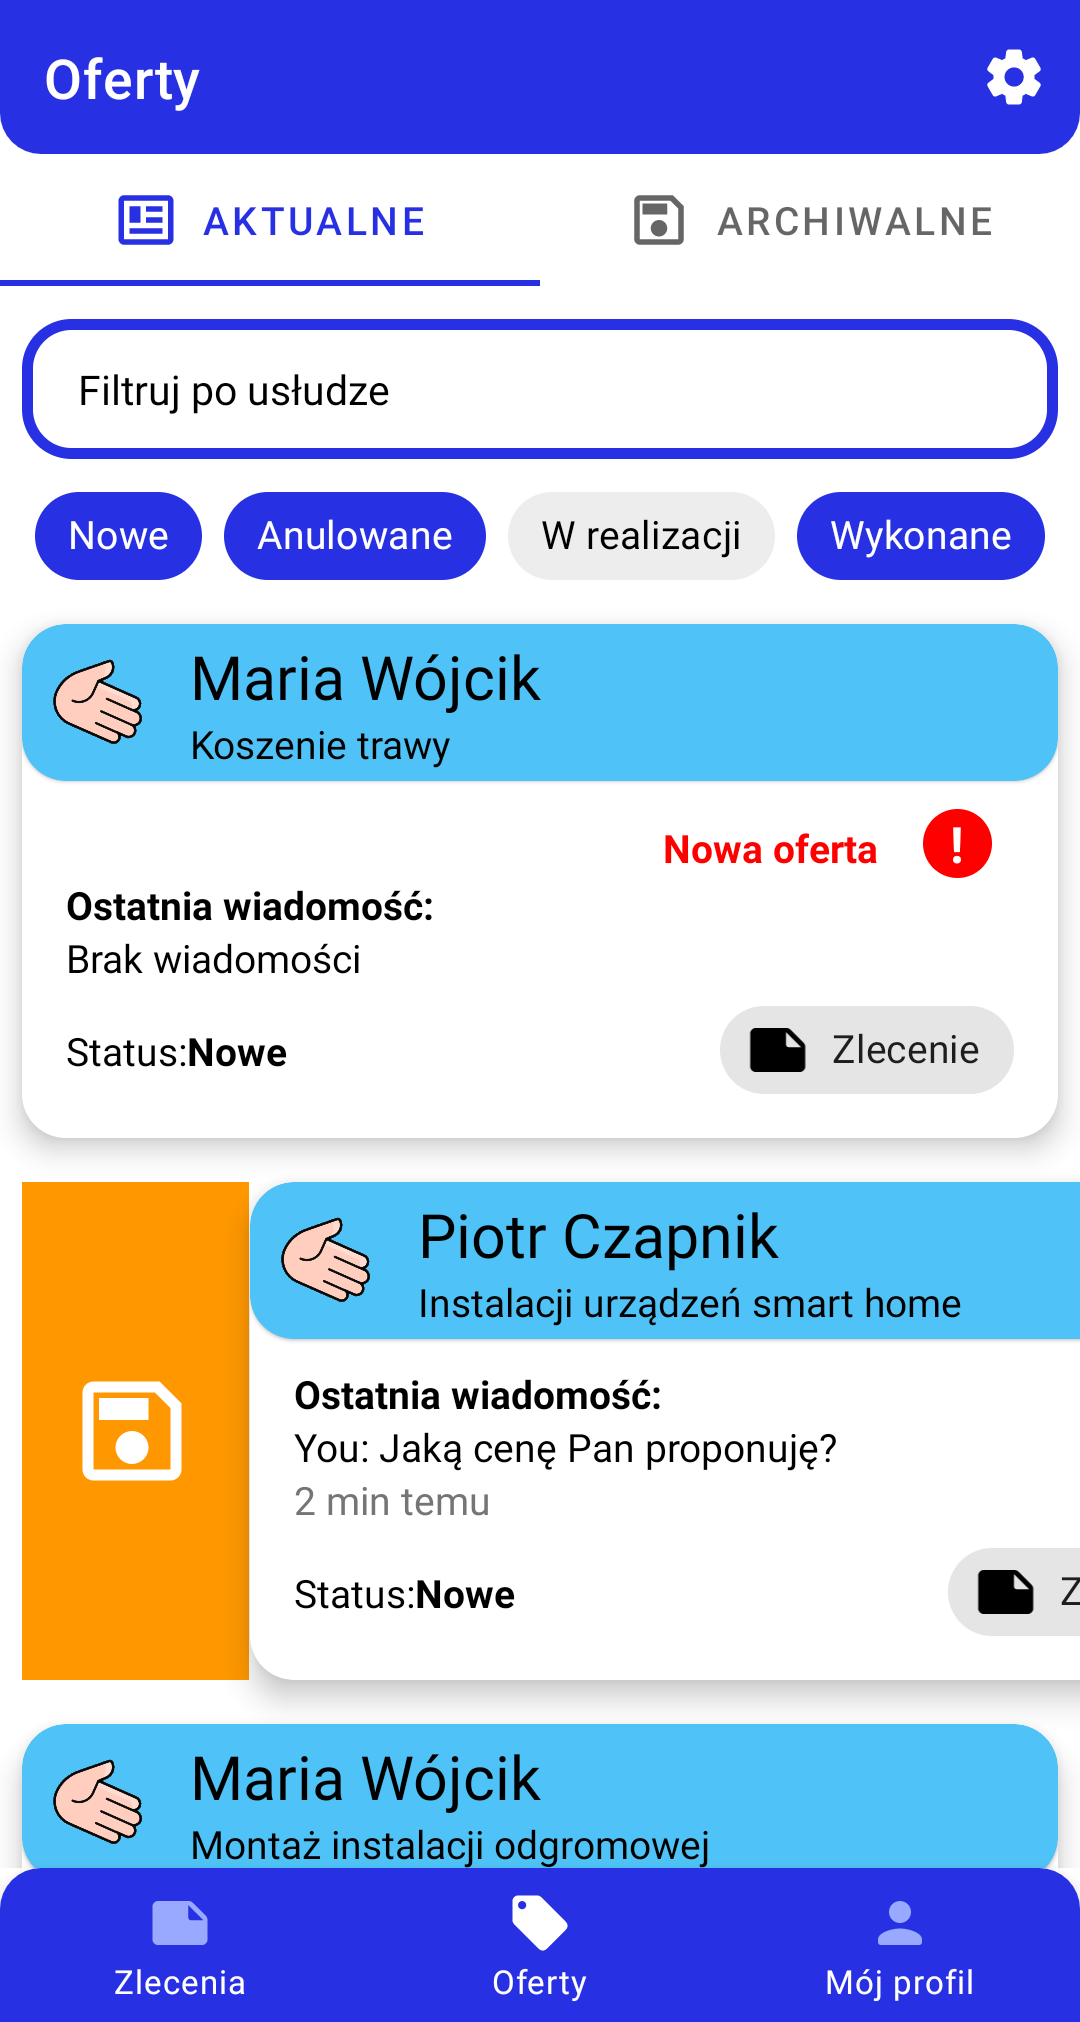
\includegraphics[width=0.97\linewidth]{screens/expert_offers_current.png}}
    \caption{Widok aktualnych ofert}
  \end{subfigure}
  \begin{subfigure}[t]{0.32\textwidth}
    \centering
    \fbox{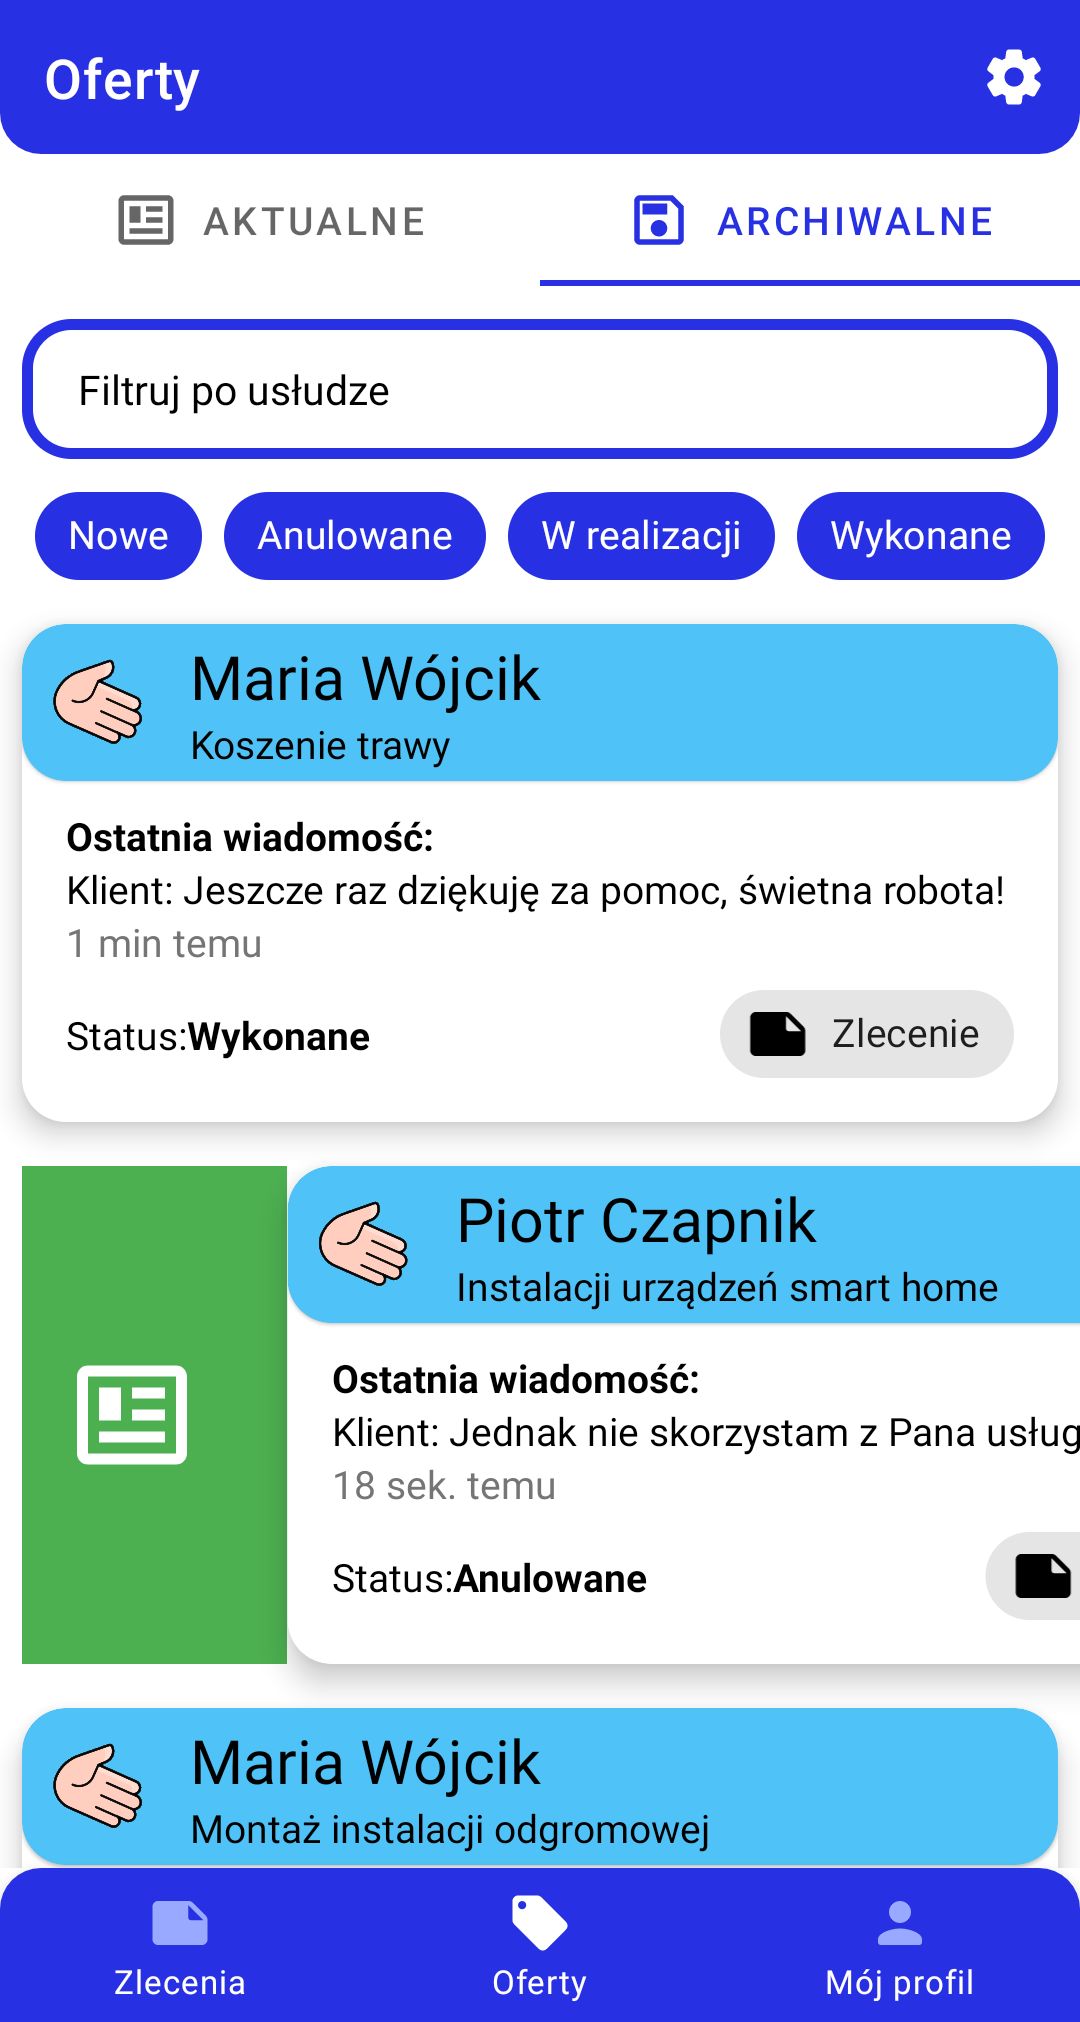
\includegraphics[width=0.97\linewidth]{screens/expert_offers_archived.png}}
    \caption{Widok archiwalnych ofert}
  \end{subfigure}
  \caption{Ekran listy złożonych przez wykonawcę ofert}
  \label{fig:offers-expert}
\end{figure}

